\normalfalse \difficiletrue \tdifficilefalse
\correctiontrue

%\UPSTIidClasse{11} % 11 sup, 12 spé
%\newcommand{\UPSTIidClasse}{11}

\exer{Pèse camion  $\star$ \label{C2:07:57:02}}
\setcounter{numques}{0}
\UPSTIcompetence[2]{C2-07}
\index{Compétence C2-07}
\index{PFS}
\index{Pèse camion}
\ifcorrection
\else
\textbf{Pas de corrigé pour cet exercice.}
\fi

\ifprof
\else
On considère un bâti \textbf{0} auquel est attaché le repère$\mathcal{R}=\left(O;\vect{x_0};\vect{y_0};\vect{z_0} \right)$. Le champ de pesanteur est $g=-g\vect{y_0}$.La barre \textbf{1} est liée au bâti \textbf{0} par une liaison pivot parfaite d’axe $\left(A,\vect{z_0}\right)$. Le plateau porte camion \textbf{2} est lié à la barre \textbf{1} par une liaison pivot parfaite d’axe $\left(C,\vect{z_0}\right)$. Le levier \textbf{3} est lié au bâti \textbf{0} par une liaison pivot parfaite d’axe $\left(B,\vect{z_0}\right)$. Ce levier est également lié au plateau \textbf{2} par une liaison pivot parfaite d’axe $\left(D,\vect{z_0}\right)$. Le camion \textbf{4}, de centre de masse $G$ et de masse $M$ inconnue, repose sur le plateau \textbf{2}.
L’action mécanique connue est caractérisée par : $\{\text{ext}\rightarrow 3\}=\left\{
\begin{array}{c}
-F\vect{y_0} \\
\vect{0} \\
\end{array}
\right\}_E$ .


\begin{center}
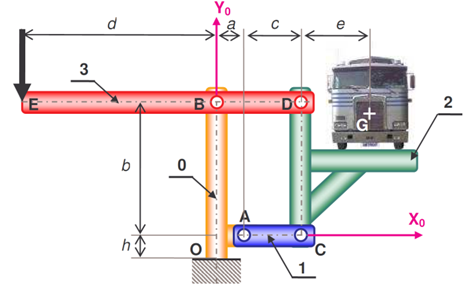
\includegraphics[width=\linewidth]{57_01}
\end{center}


\fi

\question{Tracer le graphe des liaisons en indiquant les actions mécaniques. }
\ifprof
\begin{center}
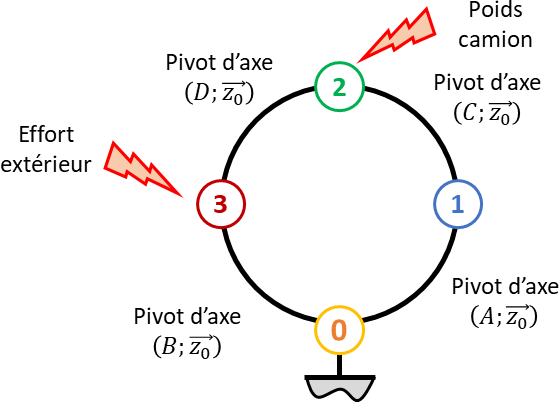
\includegraphics[width=.5\linewidth]{57_01_c}
\end{center}
\else
\fi



\question{Appliquer le PFS au solide 1.}
\ifprof
\begin{itemize}
\item On isole 1.
\item BAME :
\begin{itemize}
\item $\torseurstat{T}{0}{1}$;
\item $\torseurstat{T}{2}{1}$.
\end{itemize}
\item En utilisant l'hypothèse de problème plan, 1 est soumis à 2 glisseurs. L'action mécanique est donc orientée suivant la droite $(AC)$. 
On a donc 
$\torseurstat{T}{0}{1} = \torseurl{X_A\vect{x_0}}{\vect{0}}{A}$ et 
$\torseurstat{T}{2}{1} = \torseurl{-X_A\vect{x_0}}{\vect{0}}{C}$.

\end{itemize}
\else
\fi


\question{Appliquer le PFS au solide 2.}
\ifprof
\begin{itemize}
\item On isole 2.
\item BAME :
\begin{itemize}
\item $\torseurstat{T}{1}{2} = \torseurl{X_A\vect{x_0}}{\vect{0}}{C}$ $= \torseurl{X_A\vect{x_0}}{bX_A\vect{z_0}}{D}$;
\item $\torseurstat{T}{3}{2} = \torseurl{X_D\vect{x_0}+Y_D\vect{x_0}}{\vect{0}}{D}$;
\item $\torseurstat{T}{\text{Camion}}{2} = \torseurl{-Mg\vect{y_0}}{\vect{0}}{G}$ $ = \torseurl{-Mg\vect{y_0}}{-Mge\vect{z_0}\vect{0}}{D}$;
\end{itemize}
\item En appliquant le PFS en $D$, on a donc 
$
\left\{
\begin{array}{l}
X_A + X_D = 0 \\
Y_D = Mg \\
bX_A -Mge = 0
\end{array}
\right.$
$
\Rightarrow \left\{
\begin{array}{l}
X_D = - Mge/b \\
Y_D =  Mg \\
X_A  = Mge/b
\end{array}
\right.$
\end{itemize}
\else
\fi


\question{Appliquer le PFS au solide 3.}
\ifprof
\begin{itemize}
\item On isole 3.
\item BAME :
\begin{itemize}
\item $\torseurstat{T}{0}{3} = \torseurl{X_B\vect{x_0}+Y_B\vect{y_0}}{\vect{0}}{B}$;
\item $\torseurstat{T}{2}{3} = \torseurl{-X_D\vect{x_0}-Y_D\vect{x_0}}{\vect{0}}{D}$;
\item $\torseurstat{T}{\text{F}}{3} = \torseurl{-F\vect{y_0}}{\vect{0}}{E}$ ;
\end{itemize}
\item En appliquant le PFS en $B$, on a donc 
$
\left\{
\begin{array}{l}
X_B  - X_D = 0\\
Y_B -  Y_D -F =0 \\
Fd  - Y_D(a+c) = 0
\end{array}
\right.$
$
\Rightarrow \left\{
\begin{array}{l}
X_B  = X_D = - Mge/b  \\
Y_B = Y_D + F = Mg +F \\
Fd = Y_D(a+c) =Mg(a+c) 
\end{array}
\right.$


$F$ ne dépend de $e$ position du camion. 
\end{itemize}
\else
\fi


\question{Déterminer les actions mécaniques dans chacune des liaisons.}
\ifprof
$X_A =Mge/b$,  $X_D = - Mge/b$ et $Y_D =  Mg$, $X_B  = - Mge/b$ et $Y_B = Mg +F$. 
\else
\fi

\ifprof
\else
\begin{flushright}
\footnotesize{Corrigé voir \ref{C2:07:57:02}.}
\end{flushright}%
\fi